\section{Problem No.1} \label{sec:prob2}
\subsection{Problem Description:} 
Write programs to solve the advection equation 
$$
u_{t} + au_{x}=0,
$$
on $[0,1]$ with periodic boundary conditions using upwinding and \protect{\lw}. For smooth solutions we expect upwinding to be first-order accurate and \protect{\lw} to be second-order accurate, but it is not clear what accuracy to expect for nonsmooth solution.  
\begin{enumerate}
\item Let $a=1$ and solve the problem up to time $t=1$. Perform a refinement study for both upwinding and \protect{\lw} with $\Delta t=0.9a\Delta x$ with a smooth initial condition. Compute the rate of converge in the 1-norm and 2-norm, and max-norm. Note that the exact solution at time $t=1$ is the initial condition, and so computing the error is easy. 
\item Repeat the previous problem with the discontinuous initial condition 
$$
u(x,0) = \begin{cases}
         1\;\;\; if \;\;|x-\frac{1}{2}|<\frac{1}{4}\\
         0\;\;\; otherwise
         \end{cases}
$$
\end{enumerate}


\subsection{Solution:} 
\paragraph{Part 1:}
Under upwinding scheme, the advection equation is discretized as:
$$
\frac{u_{j}^{n+1}-u_{j}^{n}}{\Delta t} + a\frac{u_{j}^{n}-u_{j-1}^{n}}{\Delta x}=0\\
u_{j}^{n+1} = u_{j}^{n} - \frac{a\Delta t}{\Delta x}(u_{j}^{n}-u_{j-1}^{n})
$$
For which we can define \emph{Courant} number $\nu$ as $\nu = \frac{a\Delta t}{\Delta x}$.  For \protect{\lw}  scheme, the discretization would be
$$
\frac{u_{j}^{n+1}-u_{j}^{n}}{\Delta t} + a \frac{u_{j+1}^{n} -u_{j-1}^{n}}{2\Delta x} - a^2\Delta t \frac{u_{n}^{j-1}-2u_{j}^{n}+u_{j+1}^{n}}{2 \Delta x^2}=0\\
u_{j}^{n+1} = u_{j}^{n} - \frac{a \Delta t}{2\Delta x}(u_{j+1}^{n}-u_{j-1}^{n})+\frac{a^2\Delta t^2}{2\Delta x^2}(u_{j-1}^{n}-2u_{j}^{n}+u_{j+1}^{n})
$$
For smooth initial conditions we use $cos(2.0*x*PI) + sin(6.0*x*PI) / 2.0$ as initial conditions which is smooth continuous function for the periodic domain [0,1]. The periodic boundary conditions mean that the value of the last grid point is equal to the value of the first gird point. We can consider this as solving over a circle. 

Since the problem asking for solving such that $\Delta t =0.9a\Delta x$ and $a=1.0$, thus $\nu=0.9$ and the numerical scheme is stable. This applies for upwinding and \protect{\lw}. 

The error was calculated for 1-norm as $||e||_{1} = h\sum_{j}|e_{j}|$, where $e_{j}$ is the absolute difference (error) between the numerical solution and exact solution at grid point $j$. For 2-norm, the error is $||e||_{2} = h \sqrt{\sum_{j}|e_{j}|^2}$. For max-norm, the error becomes $||e||_{max}=max_{j}|e_{j}|$. 

The exact and numerical solutions for both the smooth and discontinuous initial conditions are shown in Figure \ref{fig:sol}.

\begin{figure}[!tbh]
 \centering     
   \subfloat [Smooth exact solution]{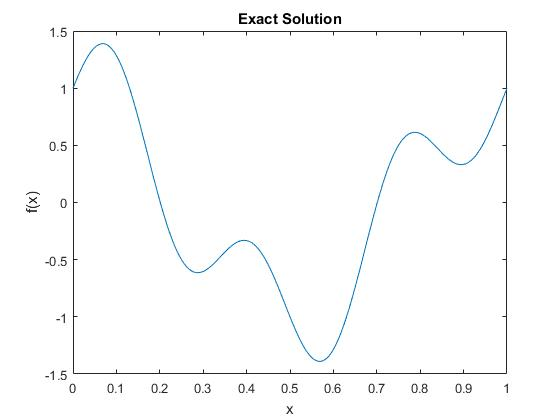
\includegraphics[width=0.3\textwidth]{fig/gt_smooth.jpg}}
   \subfloat [Smooth Upwinding solution]{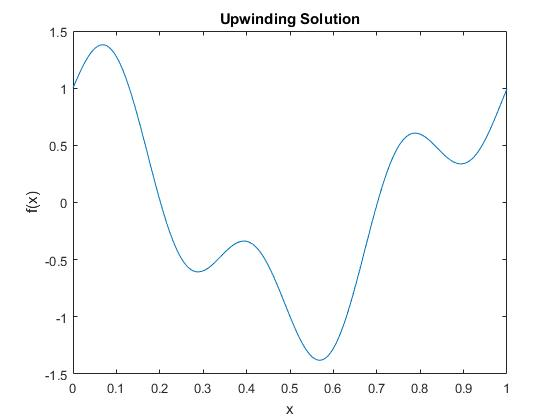
\includegraphics[width=0.3\textwidth]{fig/up_smooth.jpg}}
   \subfloat [Smooth LW solution]{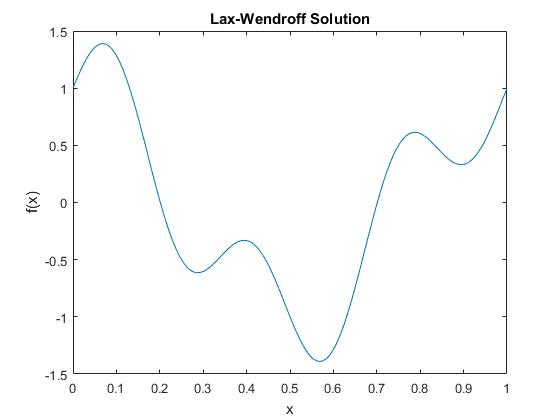
\includegraphics[width=0.3\textwidth]{fig/lw_smooth.jpg}}
   
   \subfloat [Discont. exact solution]{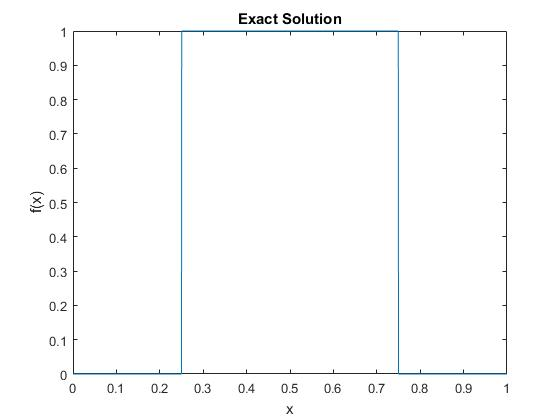
\includegraphics[width=0.3\textwidth]{fig/gt_nonsmooth.jpg}}
   \subfloat [Discont. Upwinding solution]{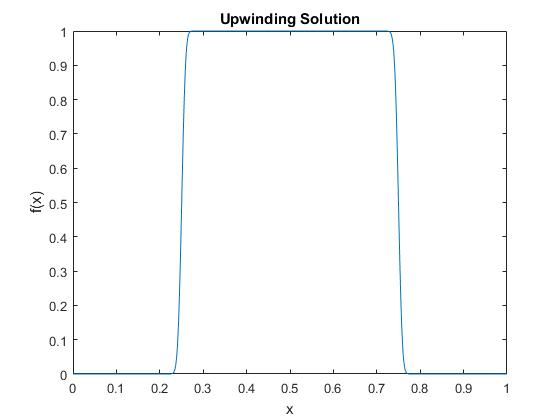
\includegraphics[width=0.3\textwidth]{fig/up_nonsmooth.jpg}}
   \subfloat [Discont. LW solution]{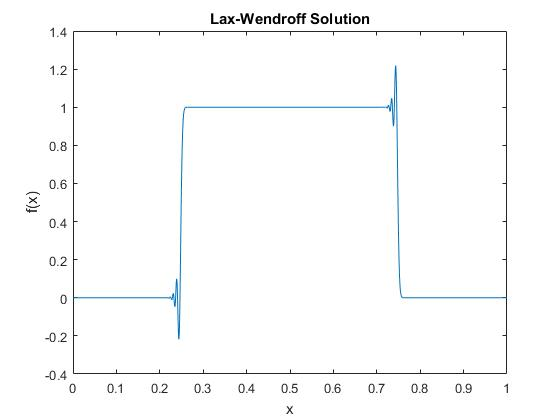
\includegraphics[width=0.3\textwidth]{fig/lw_nonsmooth.jpg}}
     \caption{The exact solution (first column), upwinding solution (second column) and \protect{\lw} solution (third column) for both smooth (first row) and discontinuous (second row) initial conditions for the 1d advection equation.}
   \label{fig:sol}
\end{figure} 
   
\begin{figure}[!tbh]
 \centering     
   \subfloat [Smooth Upwinding, 1-norm]{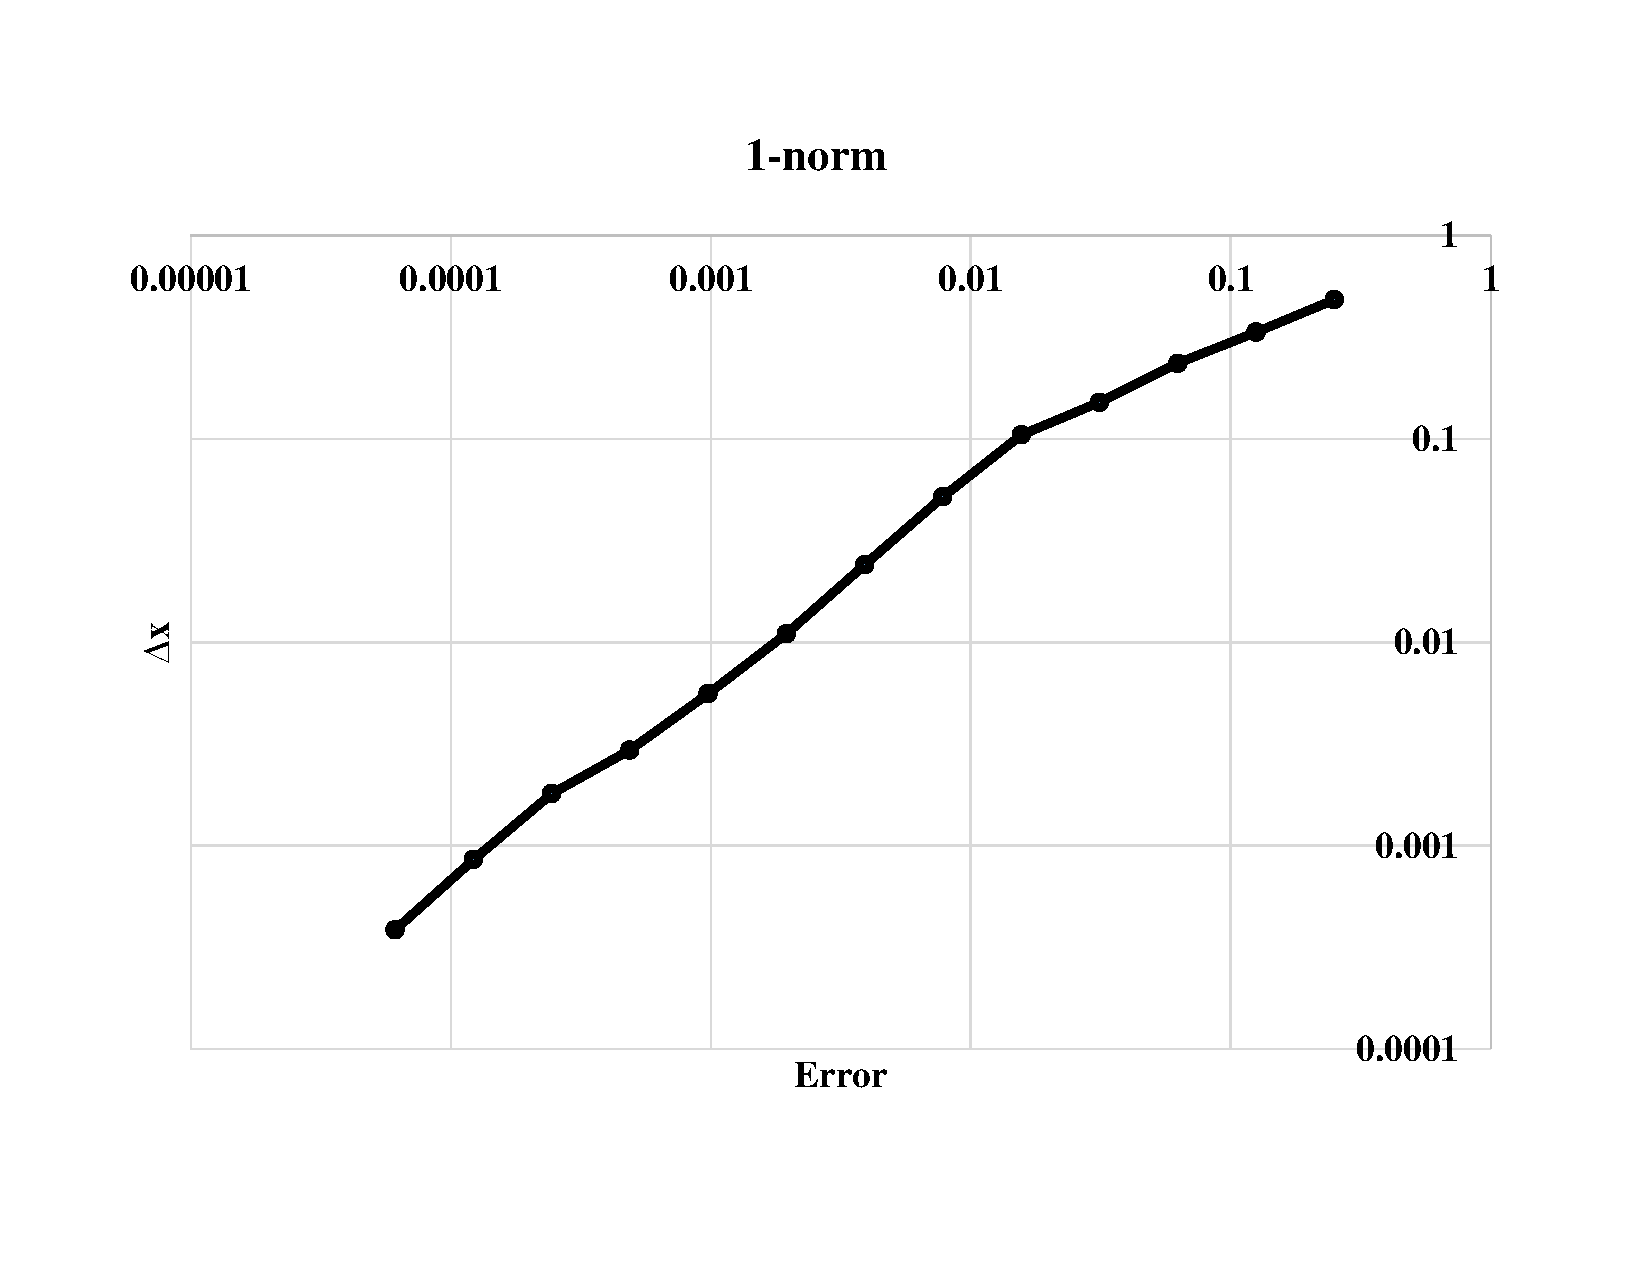
\includegraphics[width=0.3\textwidth]{fig/Up_Sm_1norm.pdf}}
   \subfloat [Smooth Upwinding, 2-norm]{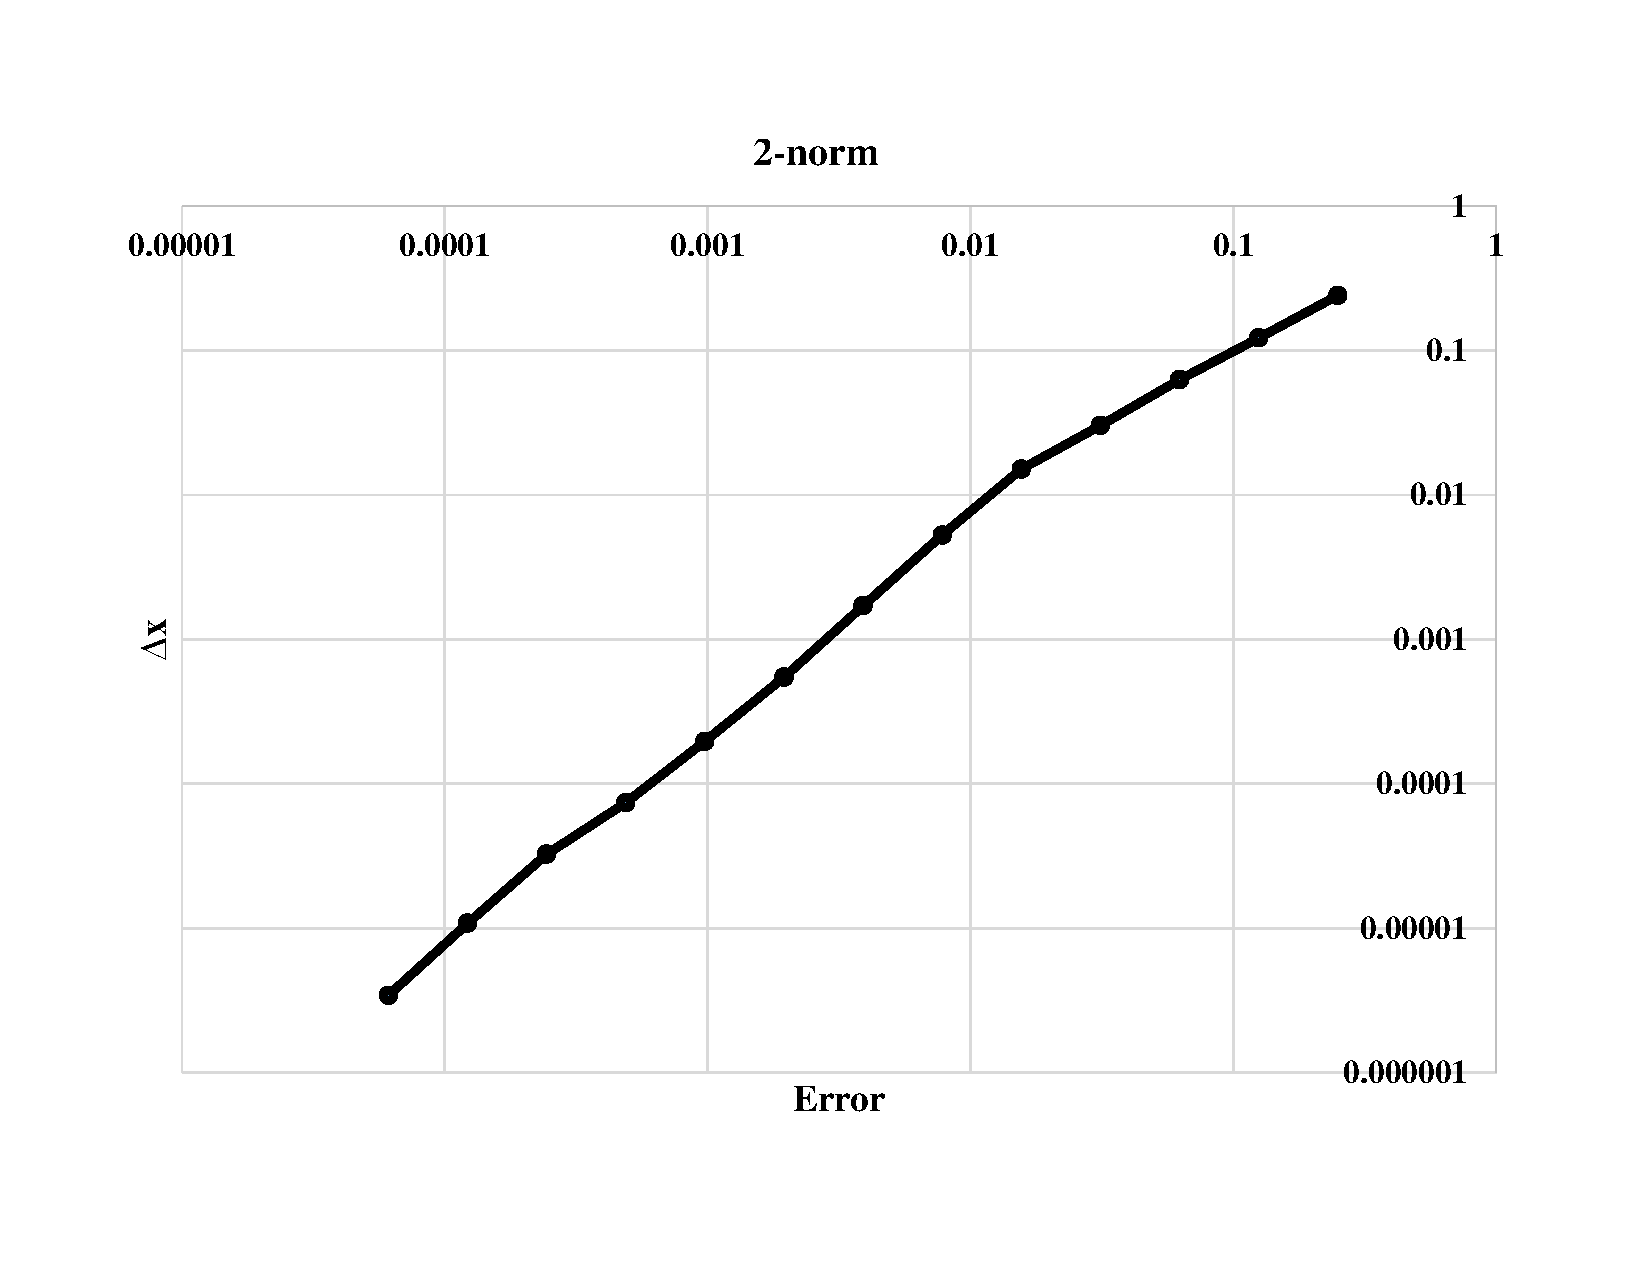
\includegraphics[width=0.3\textwidth]{fig/Up_Sm_2norm.pdf}}
   \subfloat [Smooth Upwinding, max-norm]{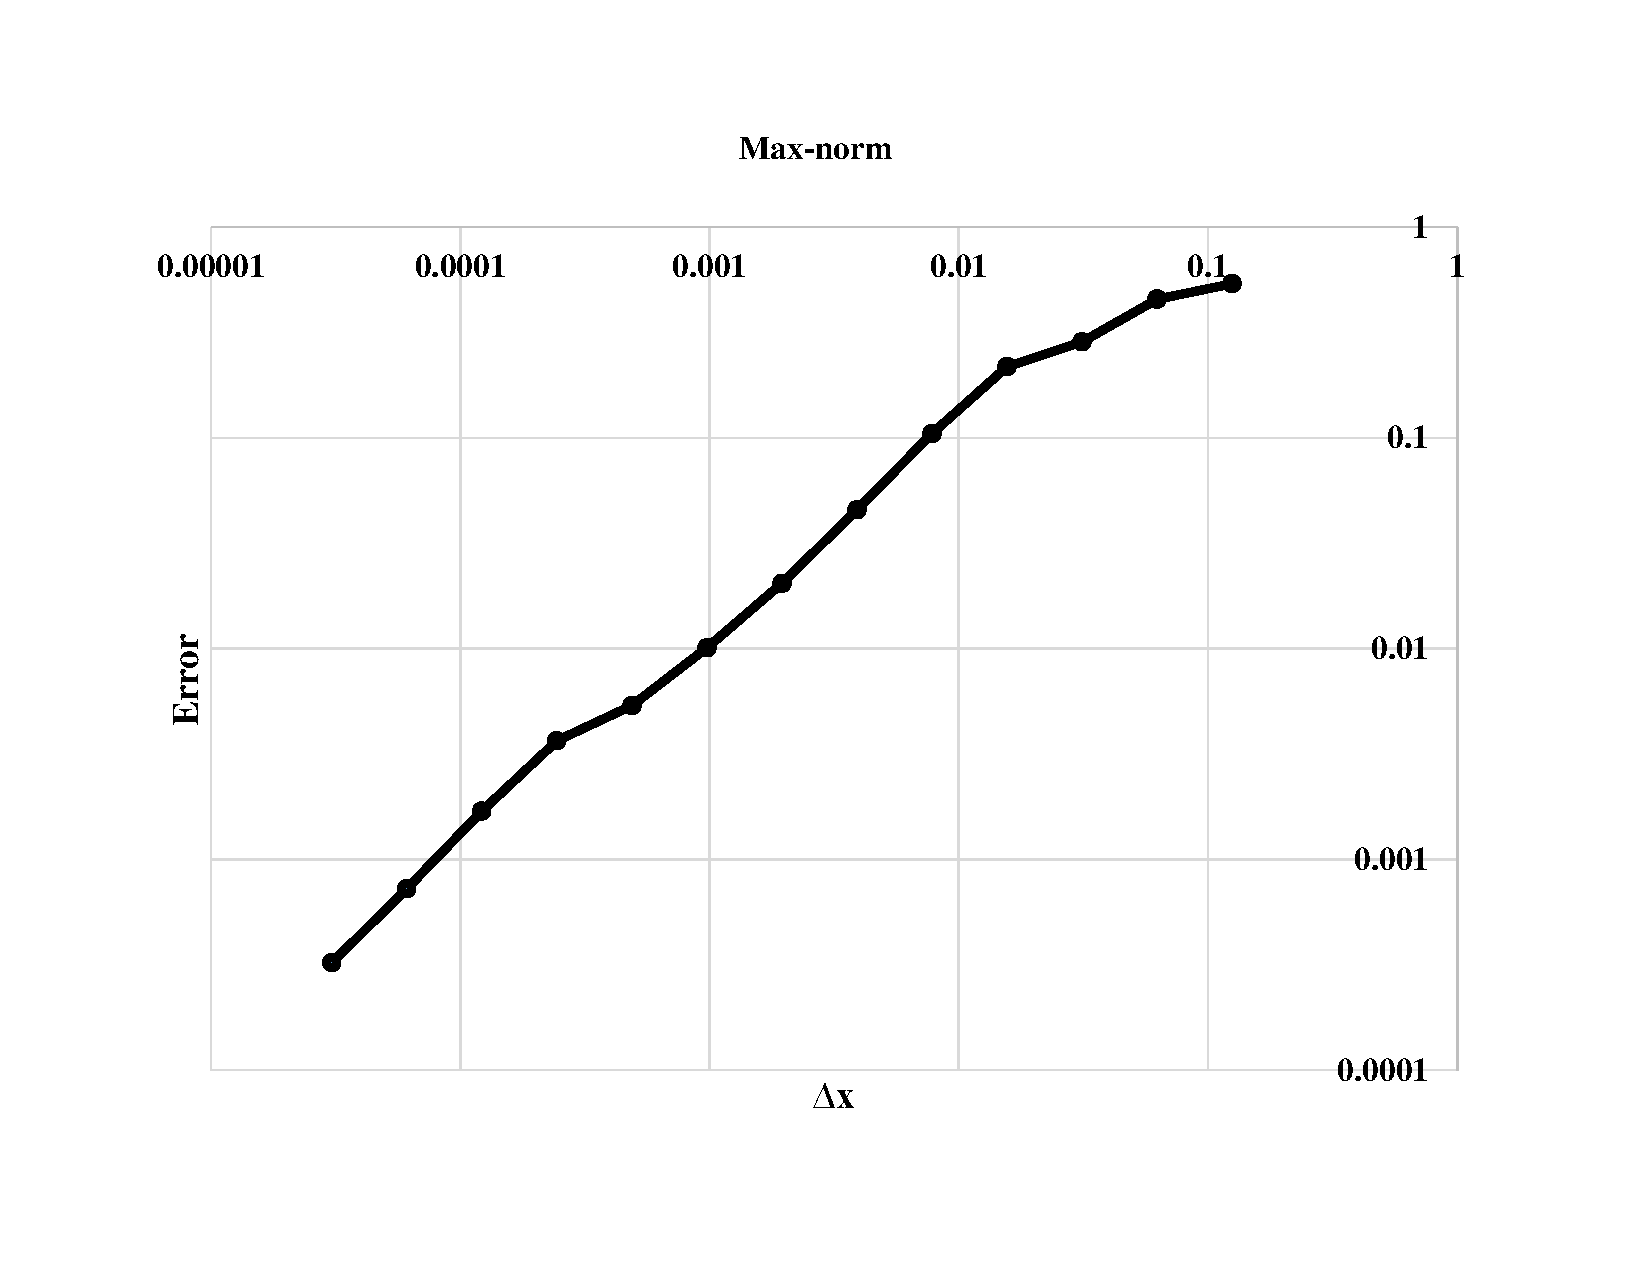
\includegraphics[width=0.3\textwidth]{fig/Up_Sm_max.pdf}}
   
   \subfloat [Smooth LW, 1-norm]{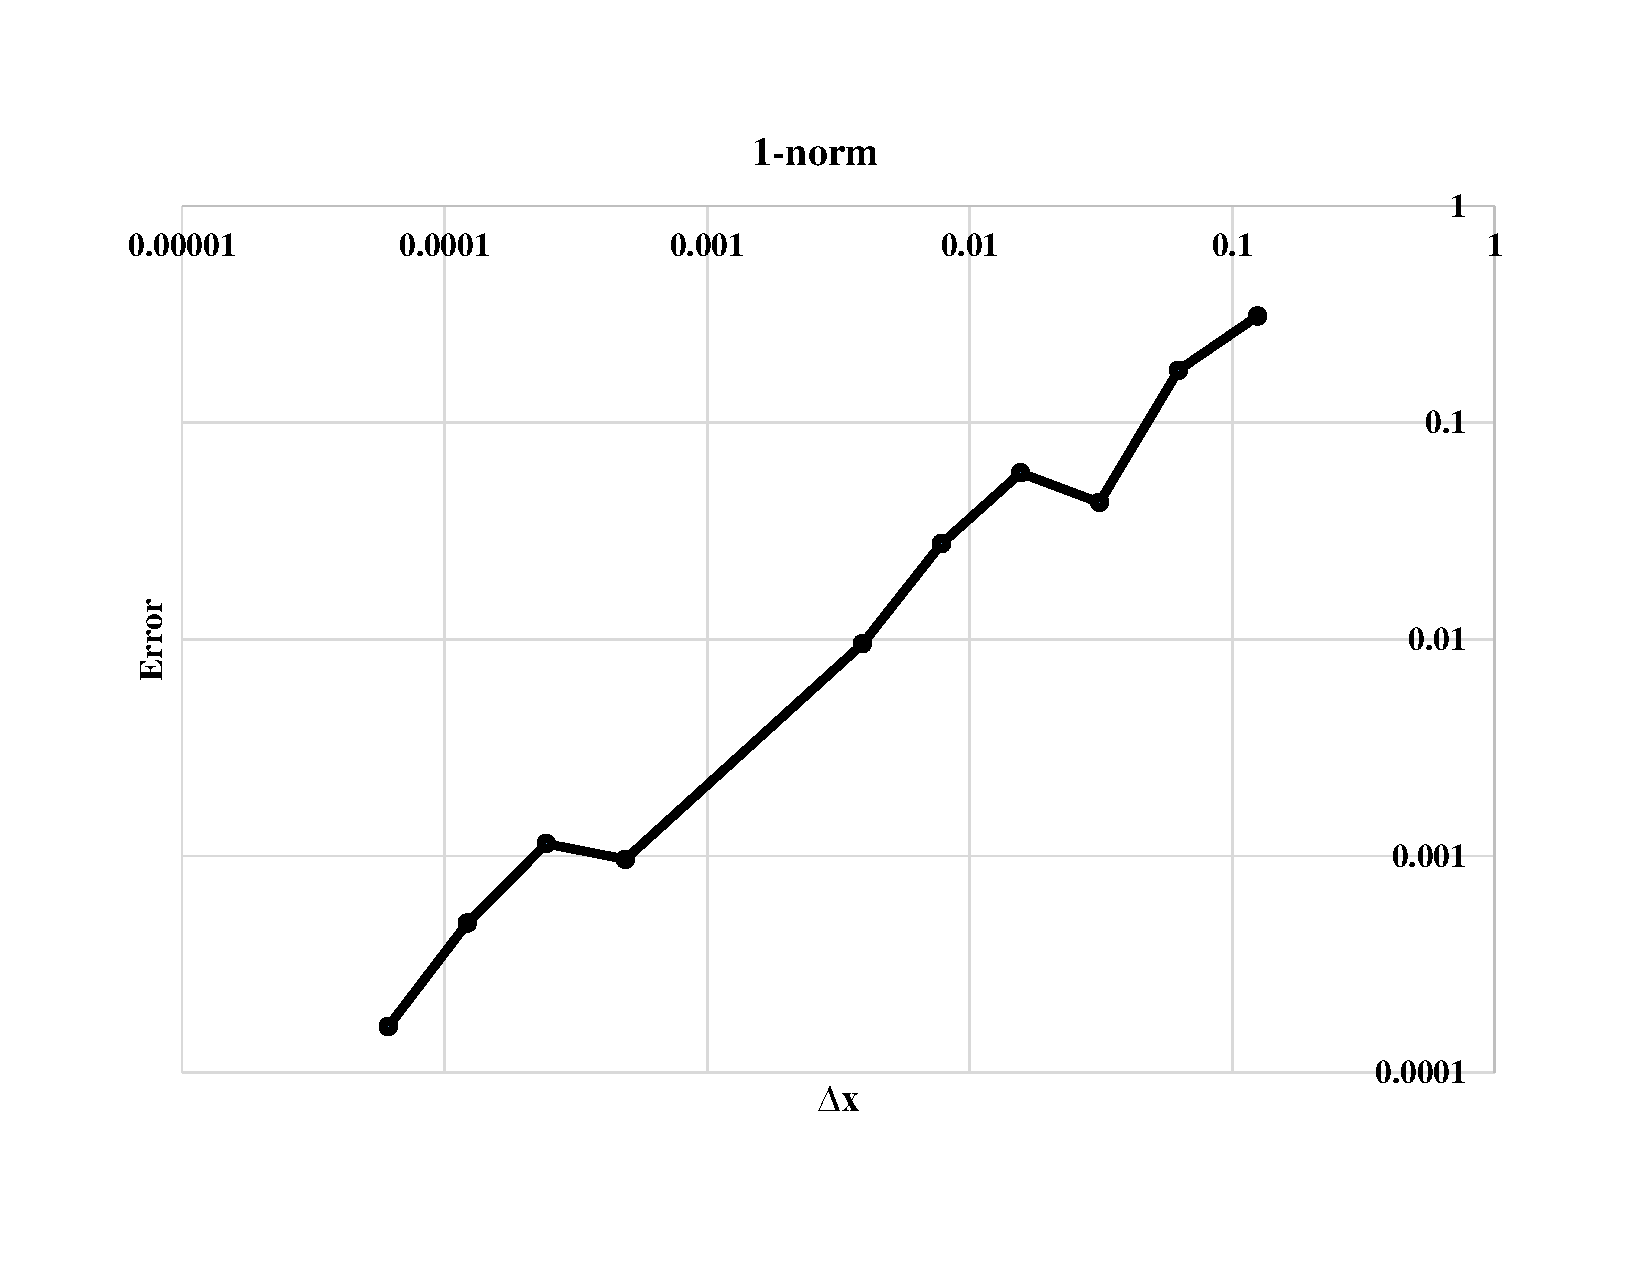
\includegraphics[width=0.3\textwidth]{fig/LW_Sm_1norm.pdf}}
   \subfloat [Smooth LW, 2-norm]{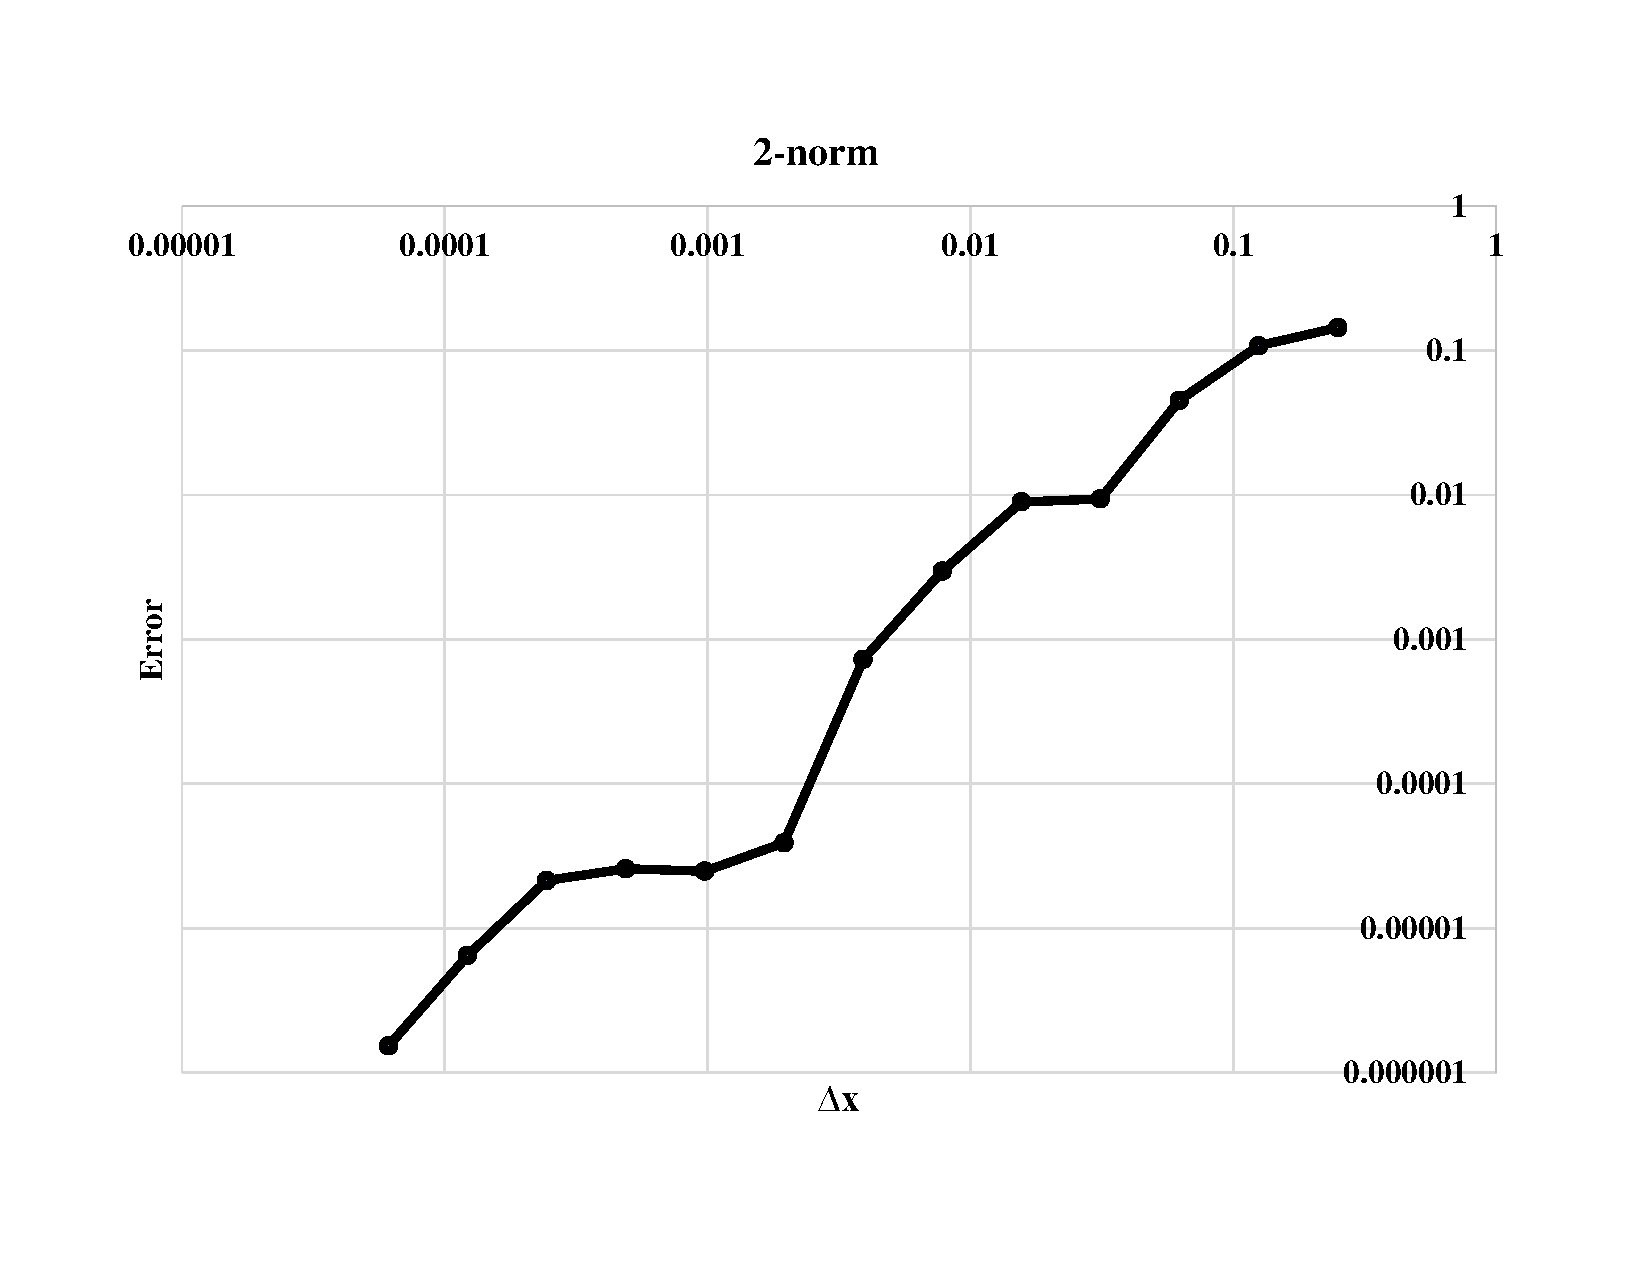
\includegraphics[width=0.3\textwidth]{fig/LW_Sm_2norm.pdf}}
   \subfloat [Smooth LW, max-norm]{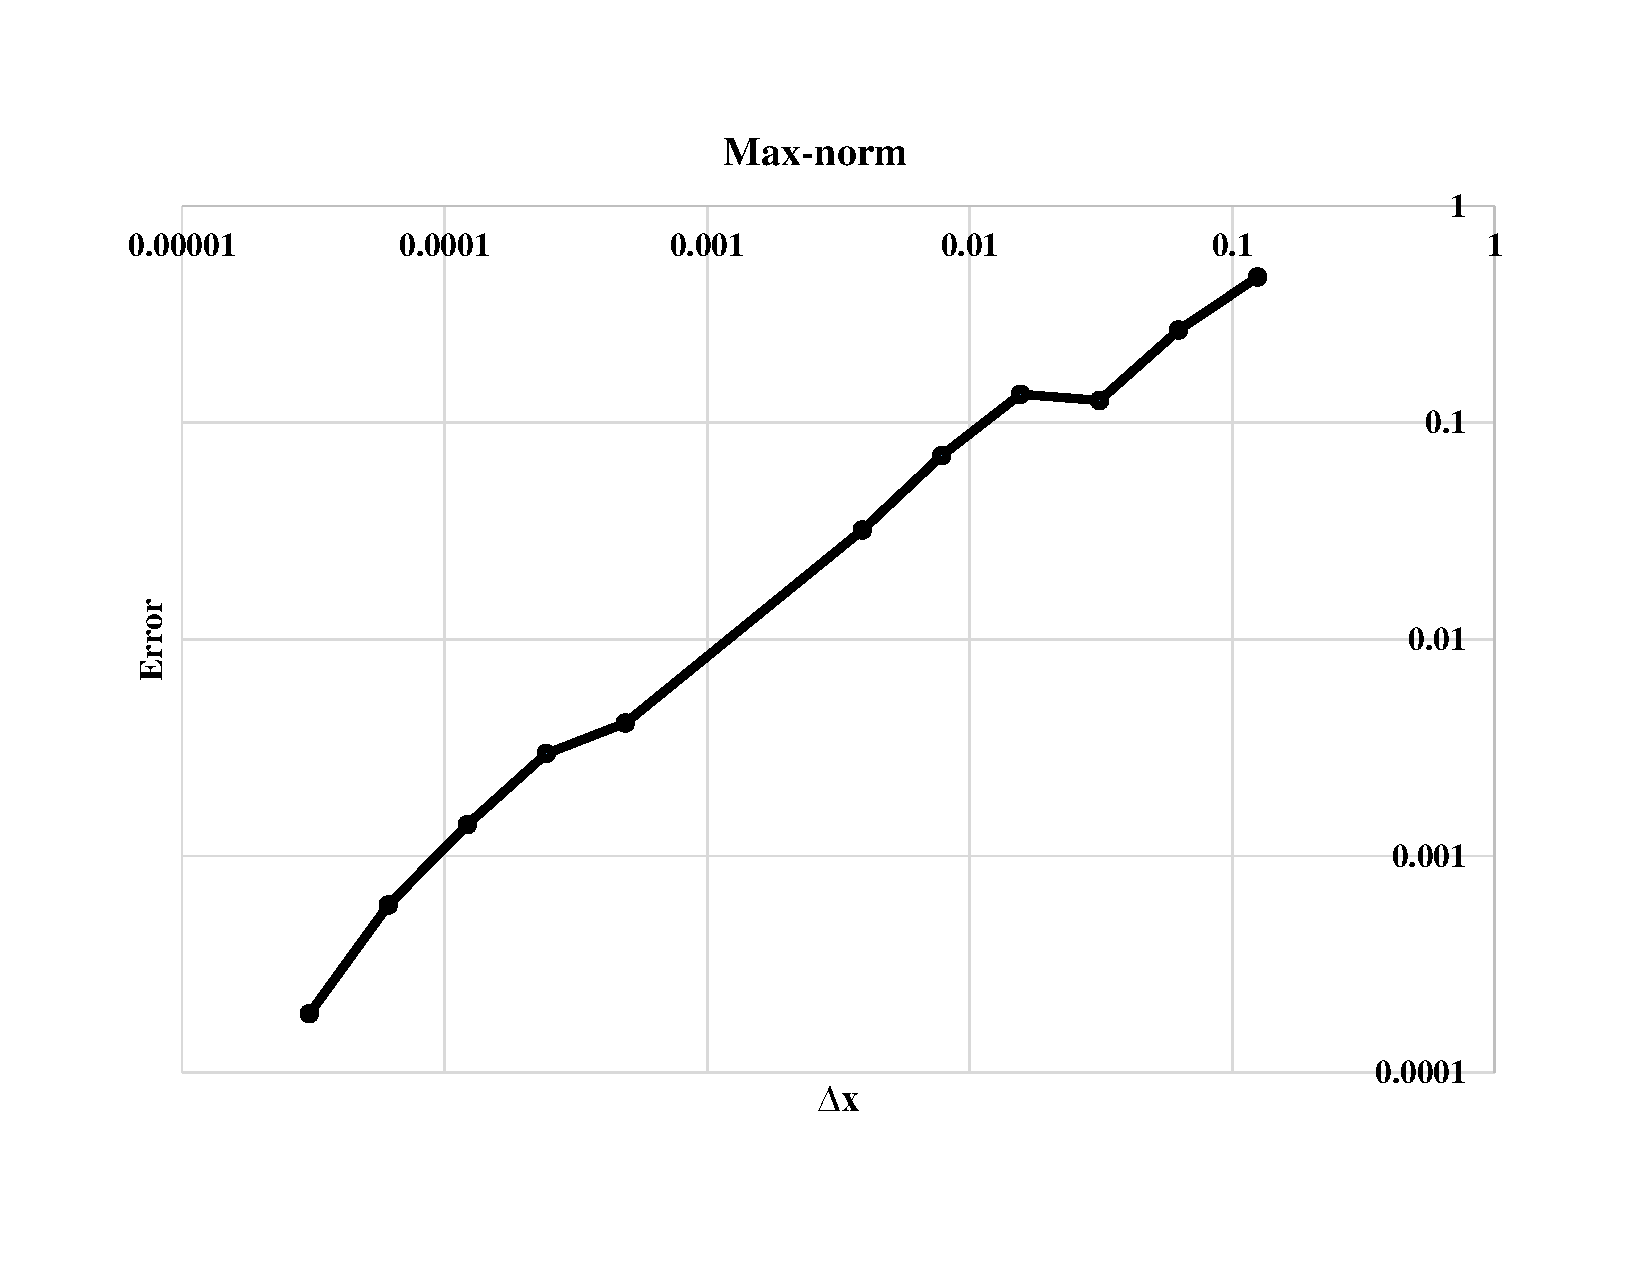
\includegraphics[width=0.3\textwidth]{fig/LW_Sm_max.pdf}}
   
   \subfloat [Discont. Upwinding, 1-norm]{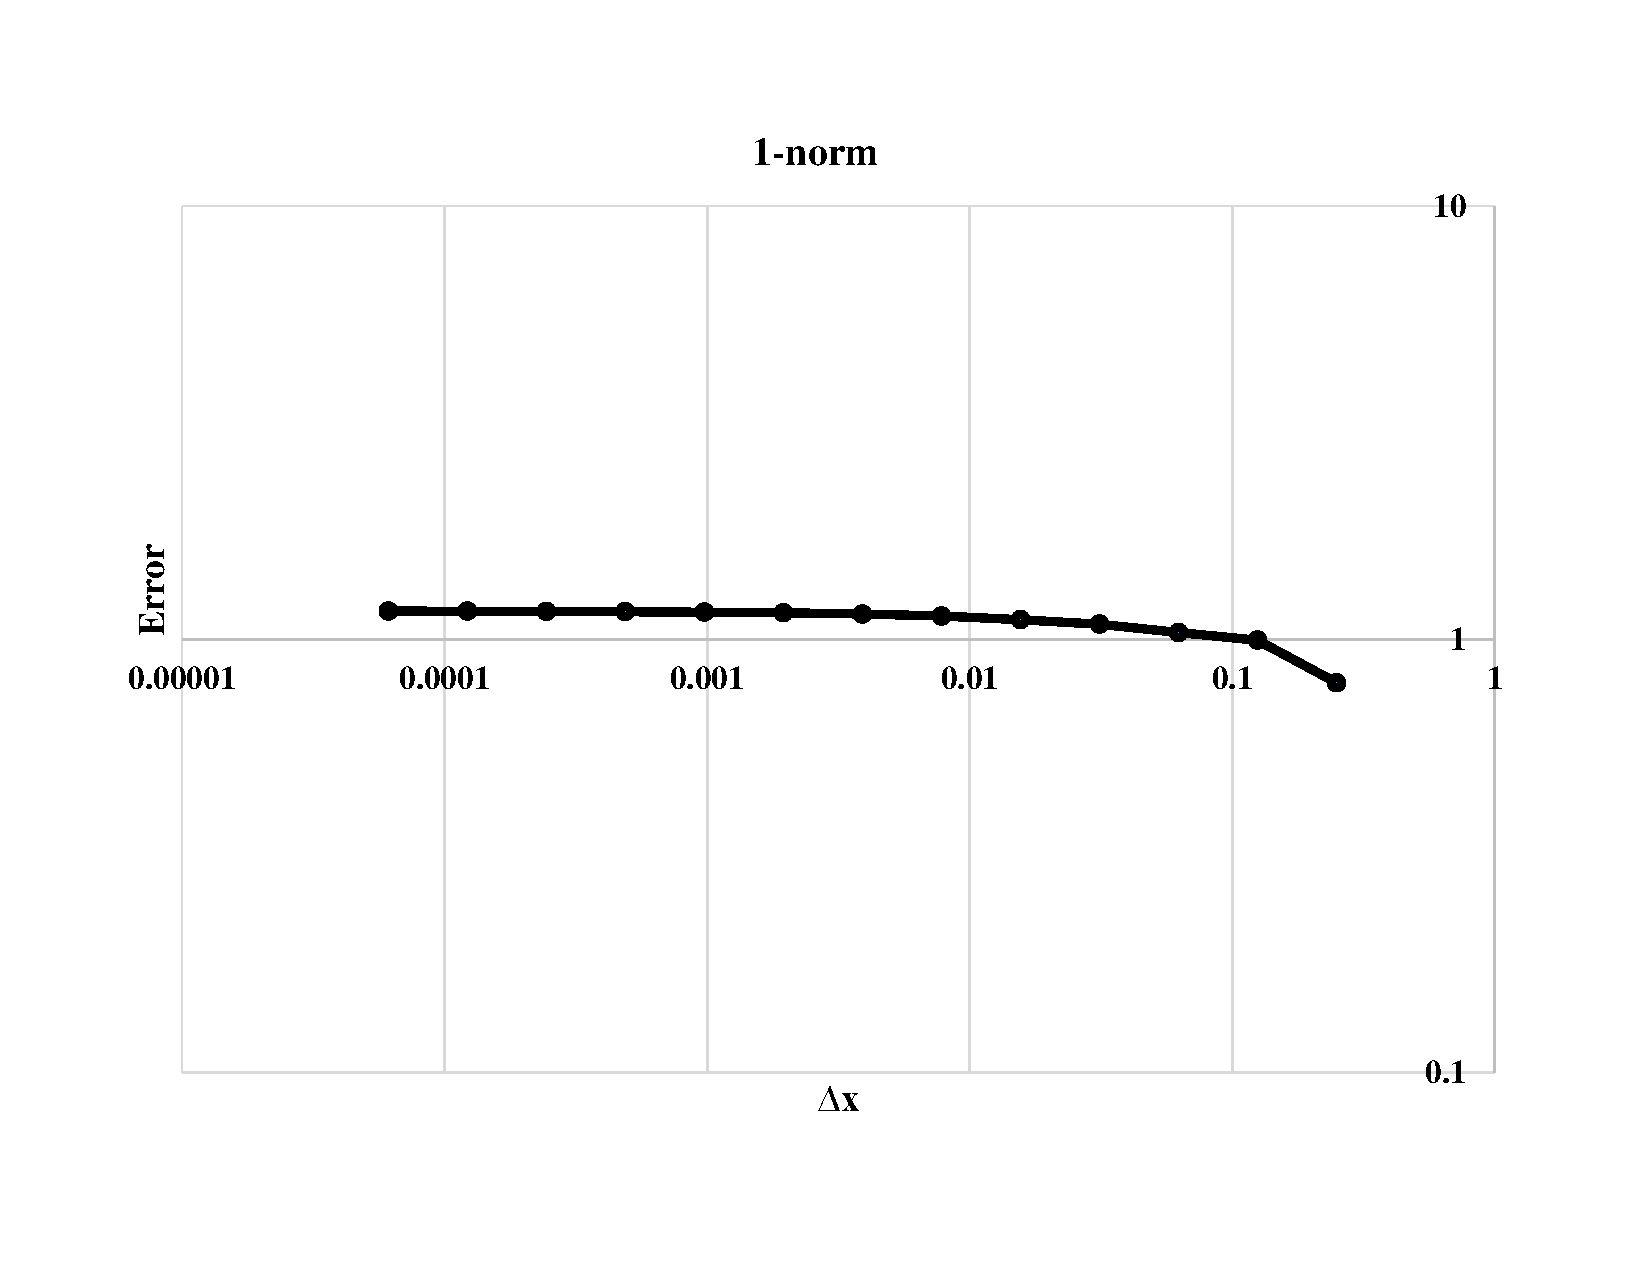
\includegraphics[width=0.3\textwidth]{fig/Up_NonSm_1norm.pdf}}
   \subfloat [Discont. Upwinding, 2-norm]{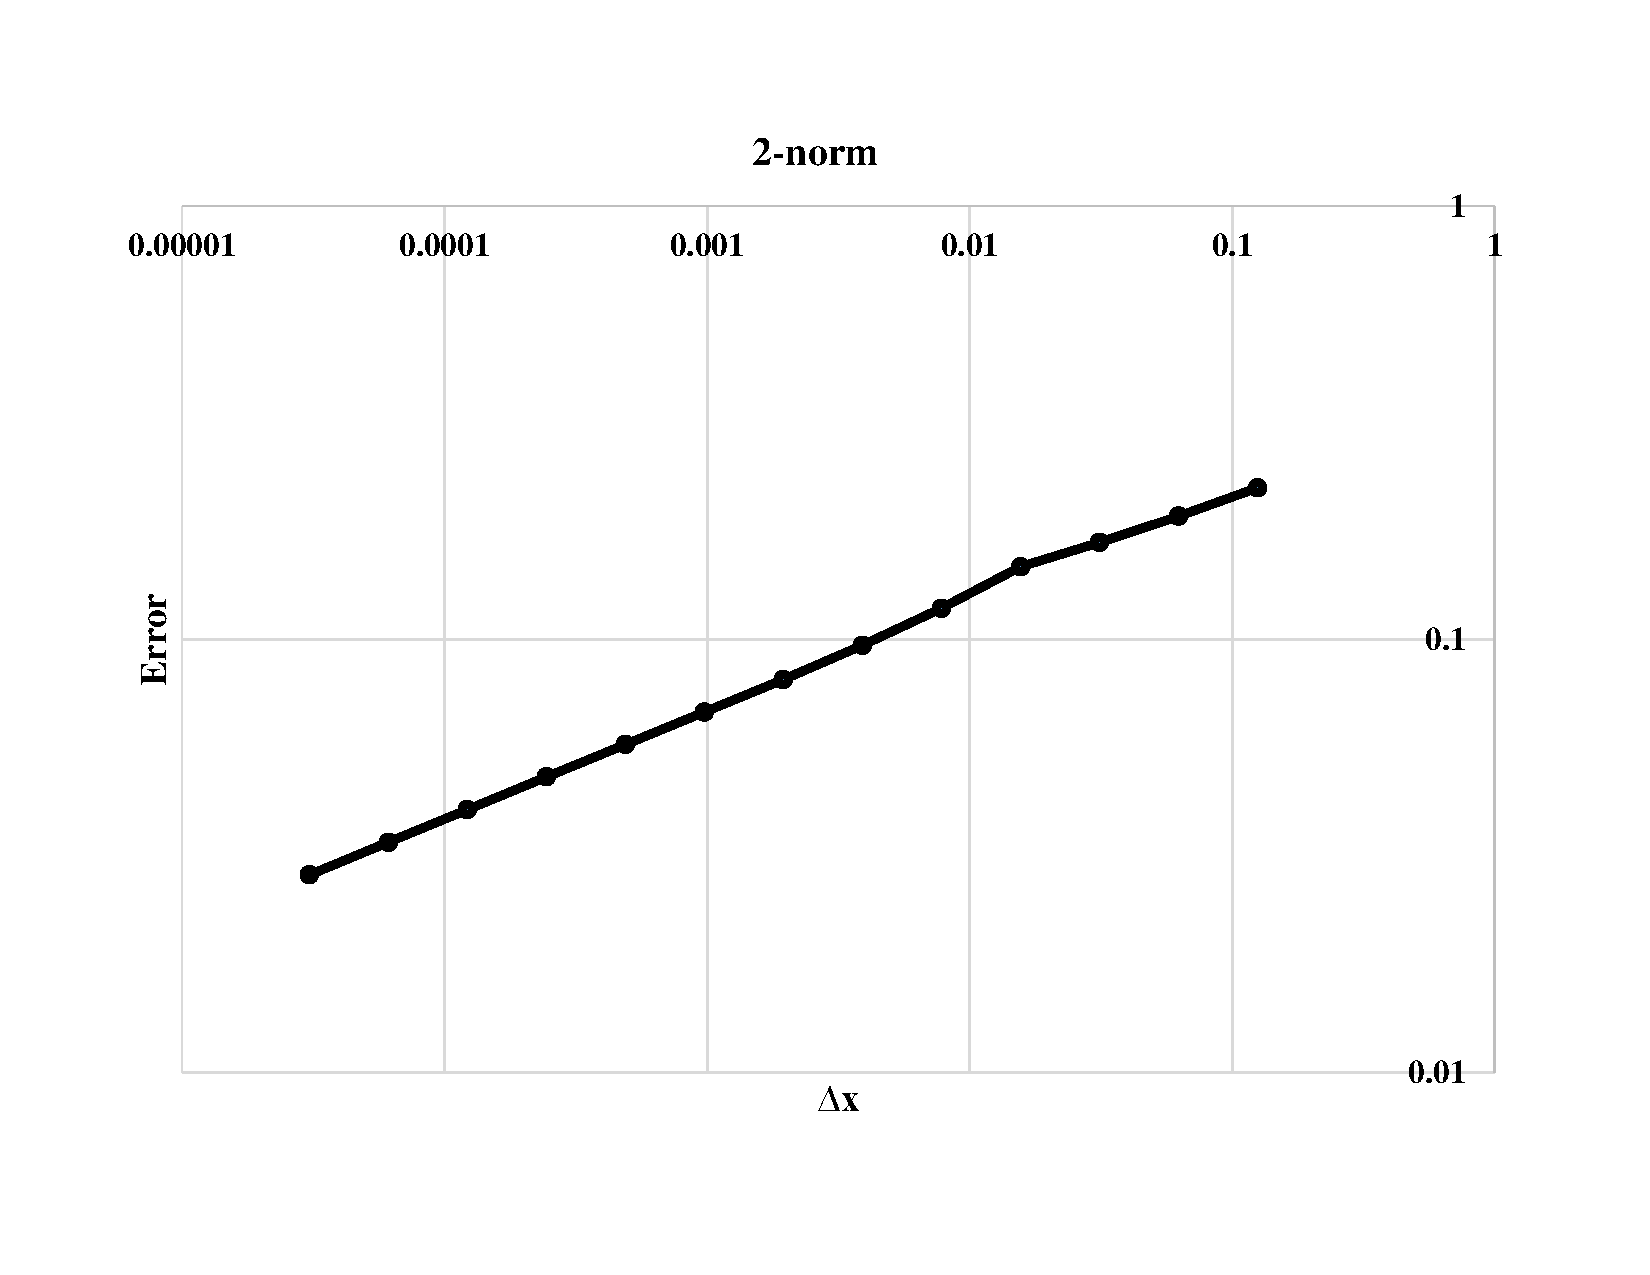
\includegraphics[width=0.3\textwidth]{fig/Up_NonSm_2norm.pdf}}
   \subfloat [Discont. Upwinding, max-norm]{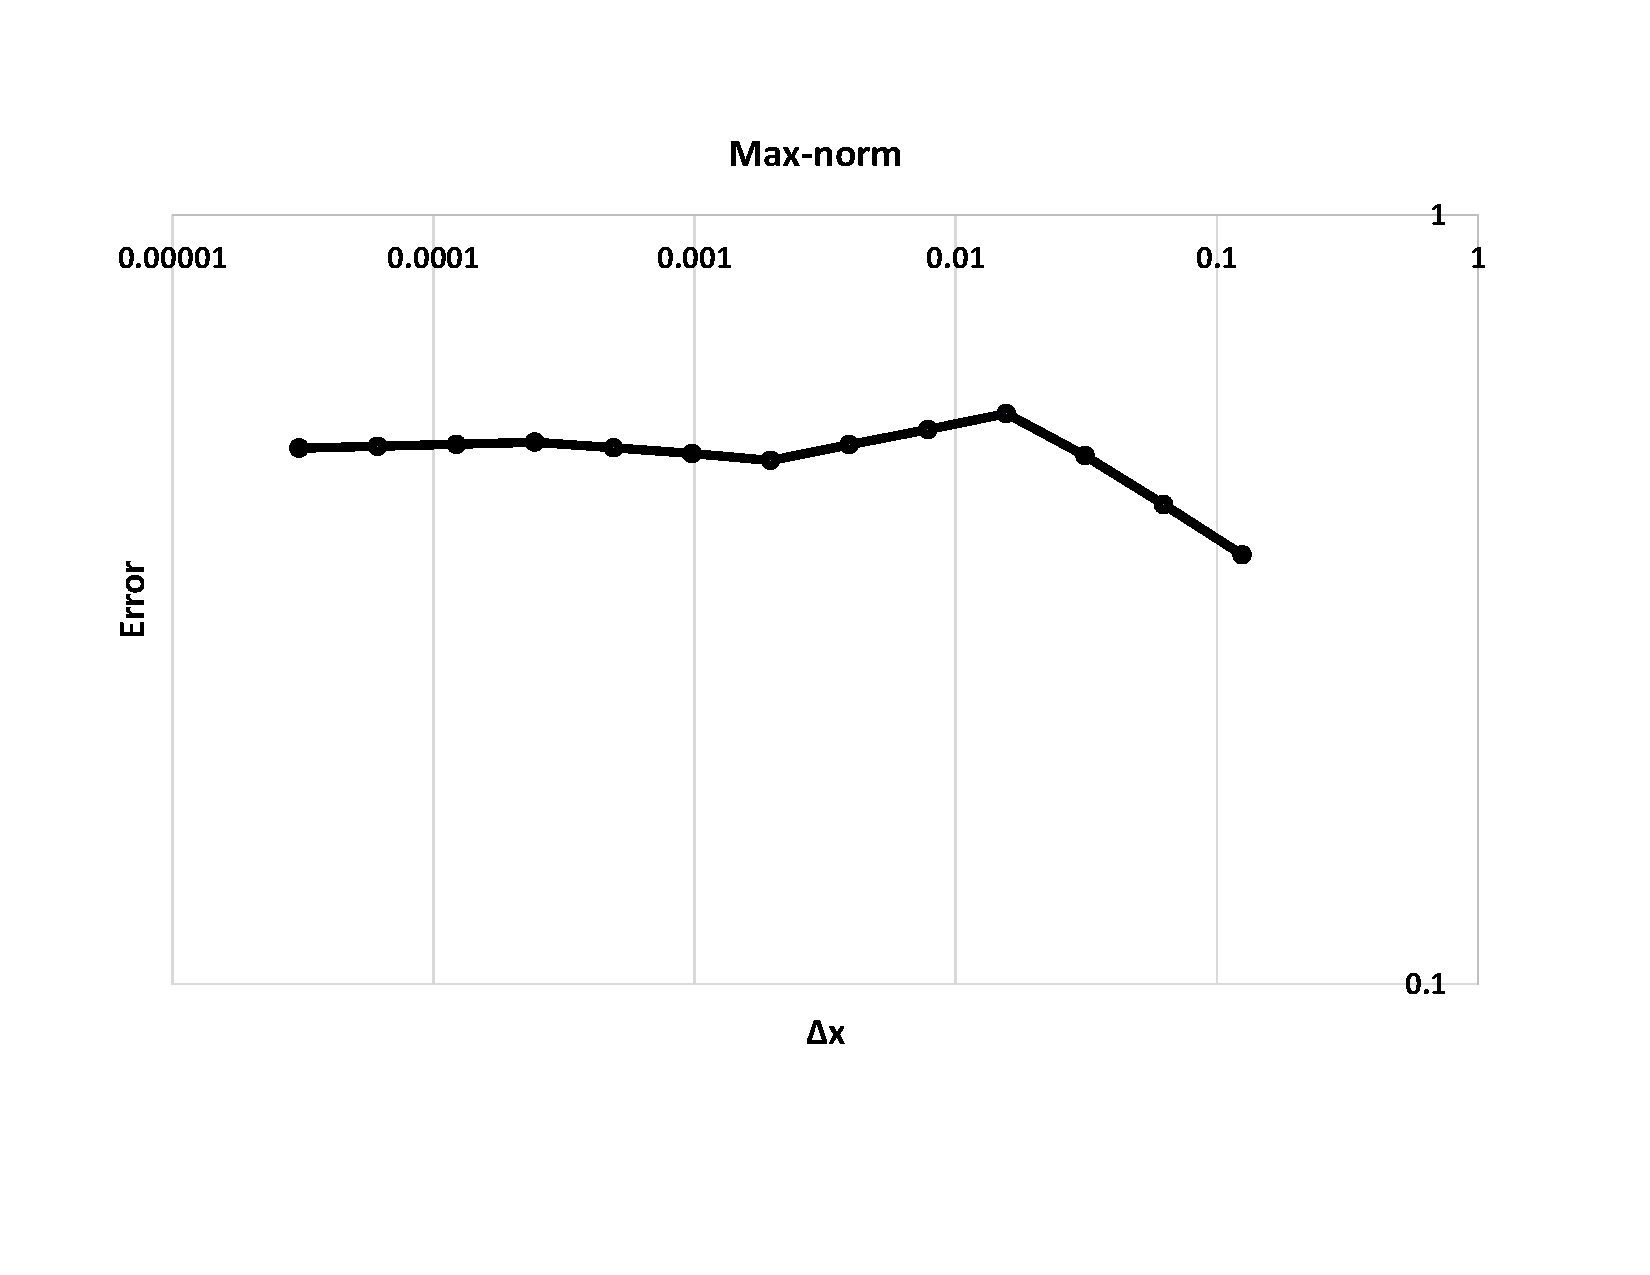
\includegraphics[width=0.3\textwidth]{fig/Up_NonSm_max.pdf}} 
   
   \subfloat [Discont. LW, 1-norm]{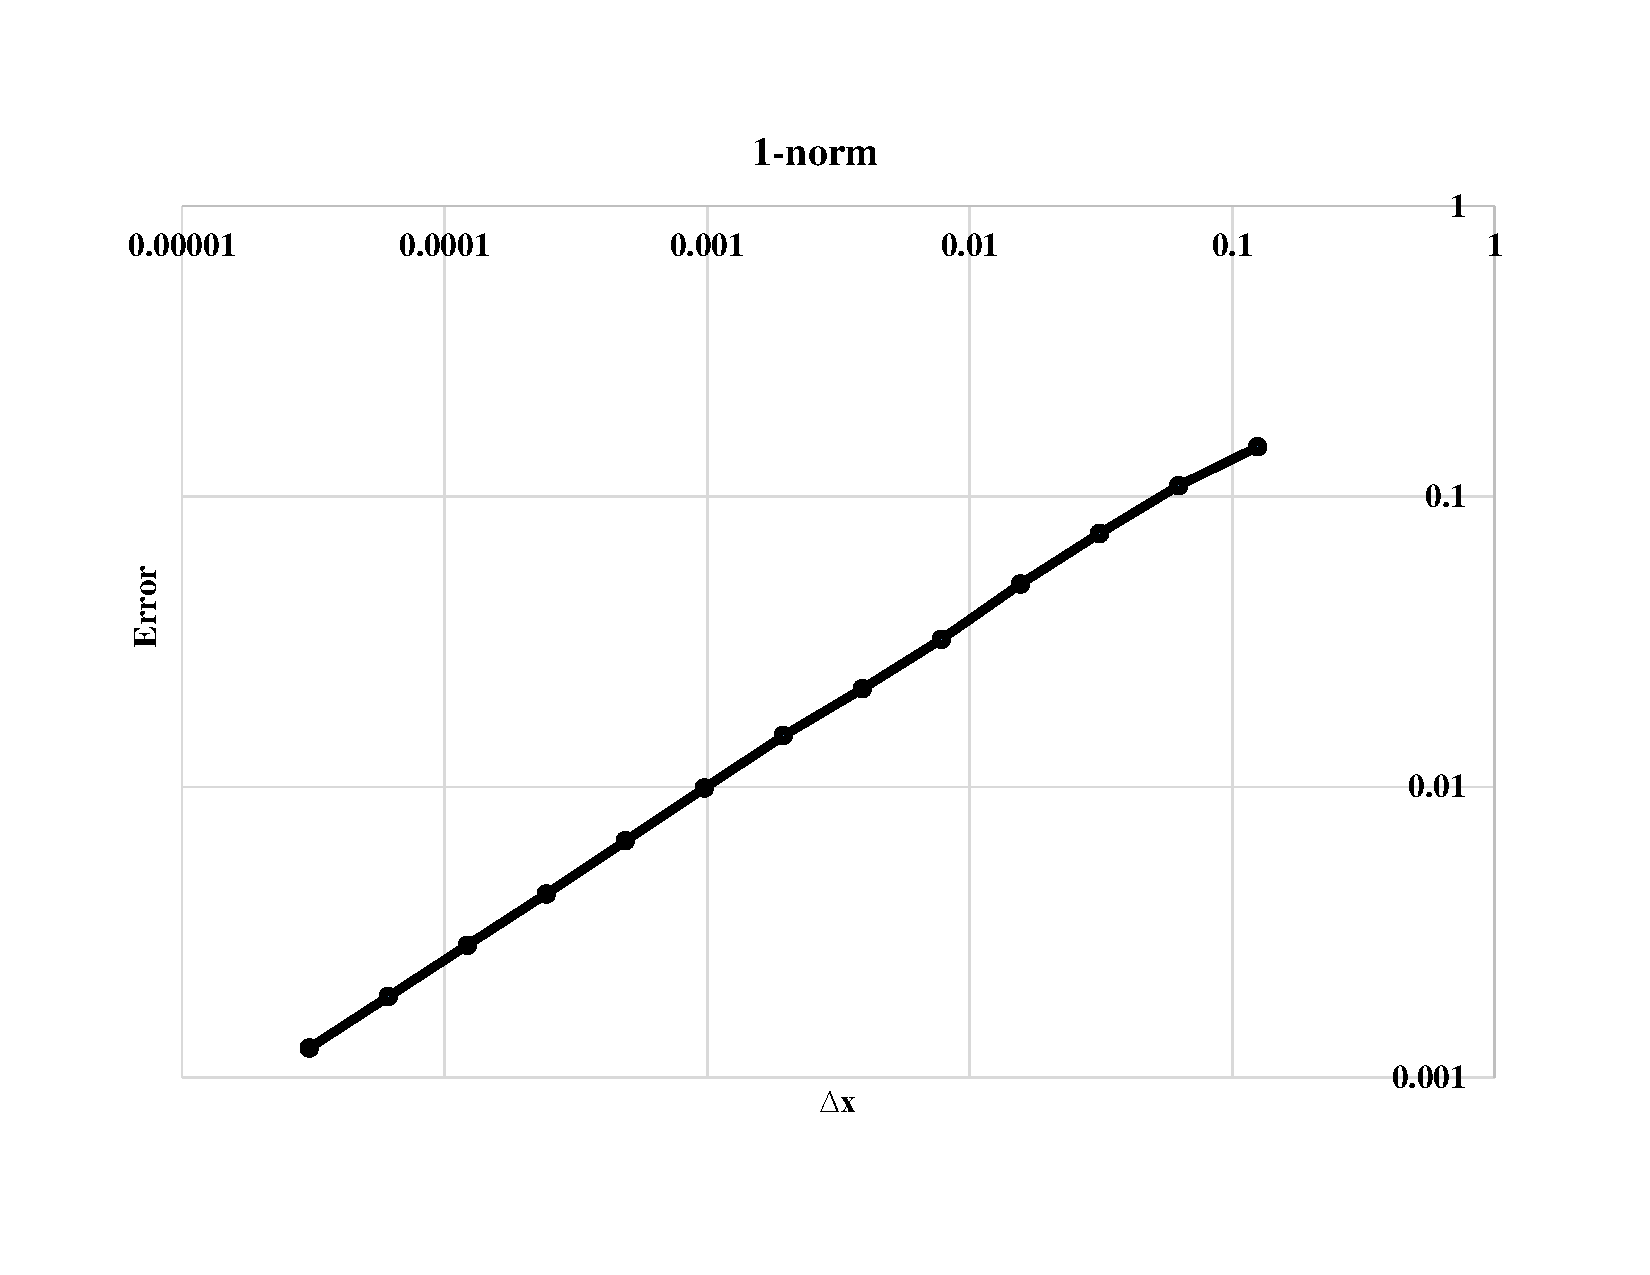
\includegraphics[width=0.3\textwidth]{fig/LW_NonSm_1norm.pdf}}
   \subfloat [Discont. LW, 2-norm]{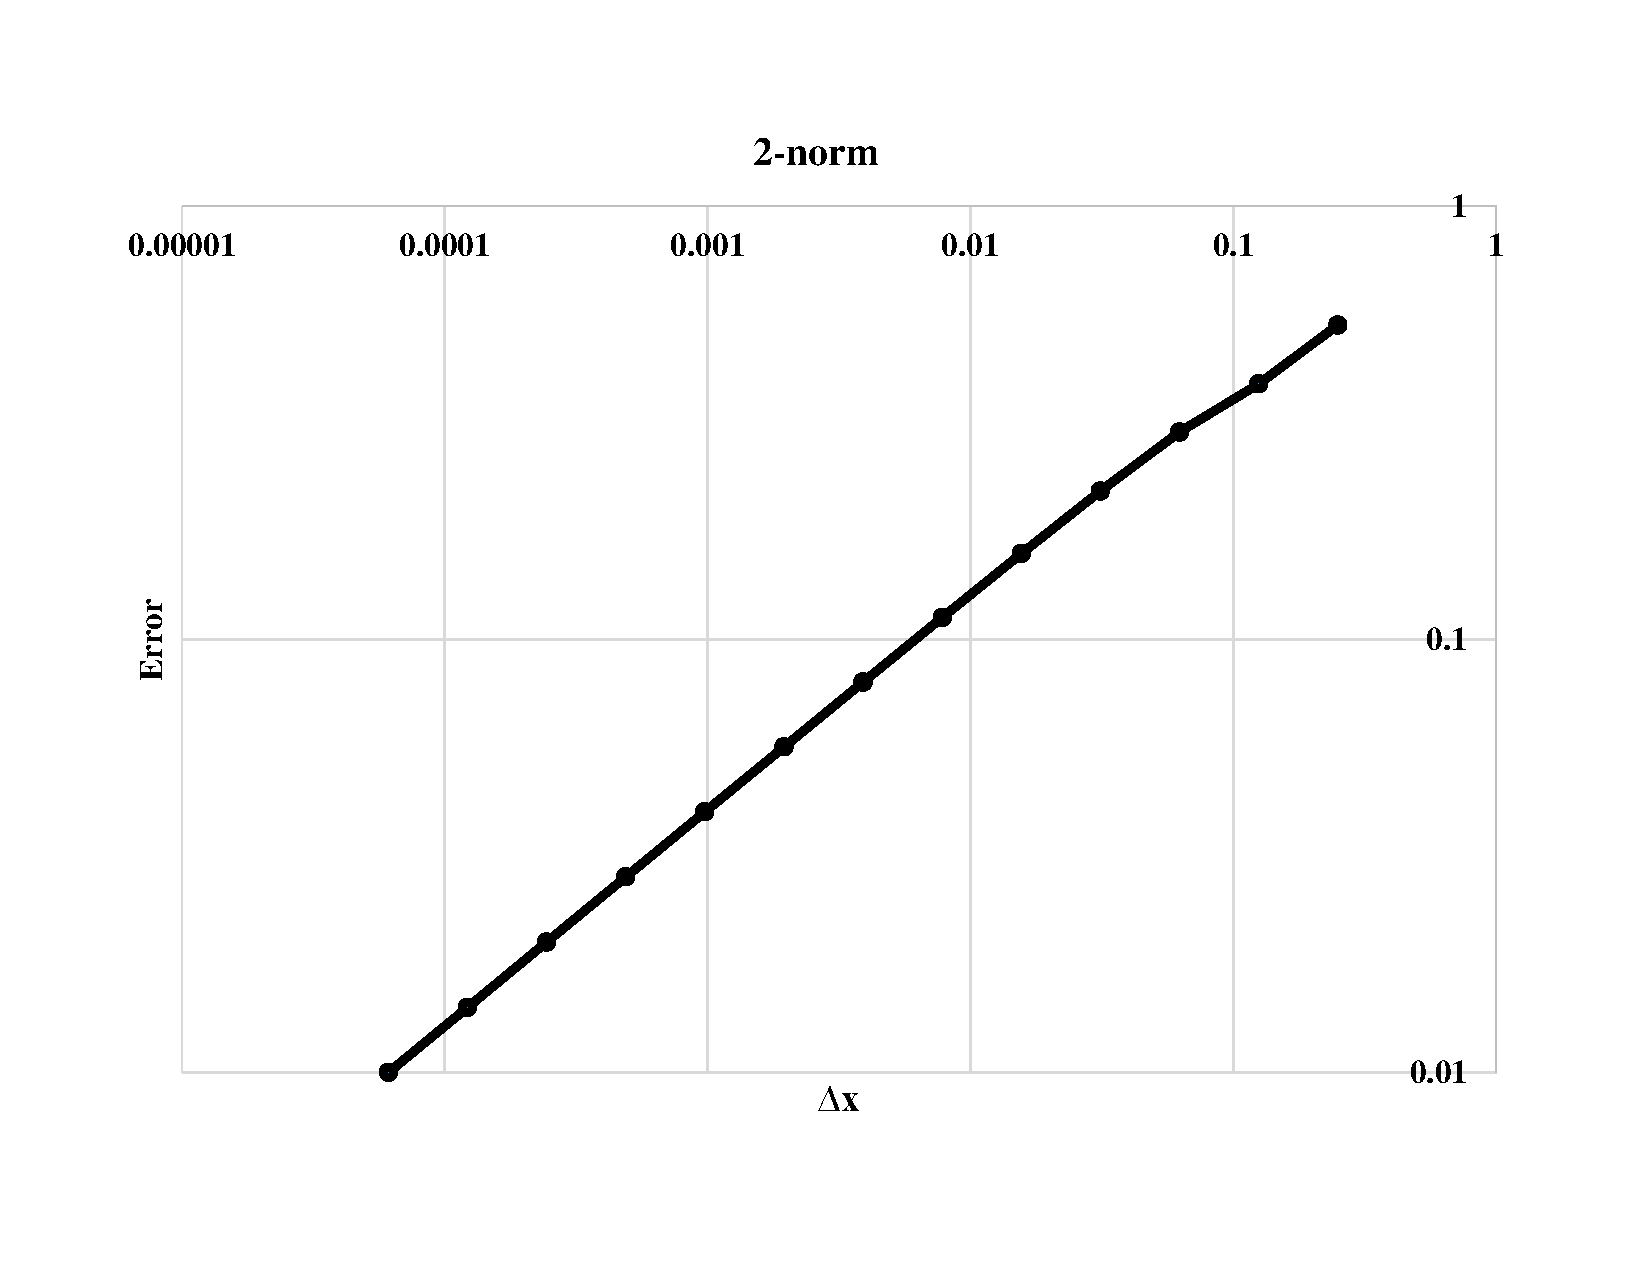
\includegraphics[width=0.3\textwidth]{fig/LW_NonSm_2norm.pdf}}
   \subfloat [Discont. LW, max-norm]{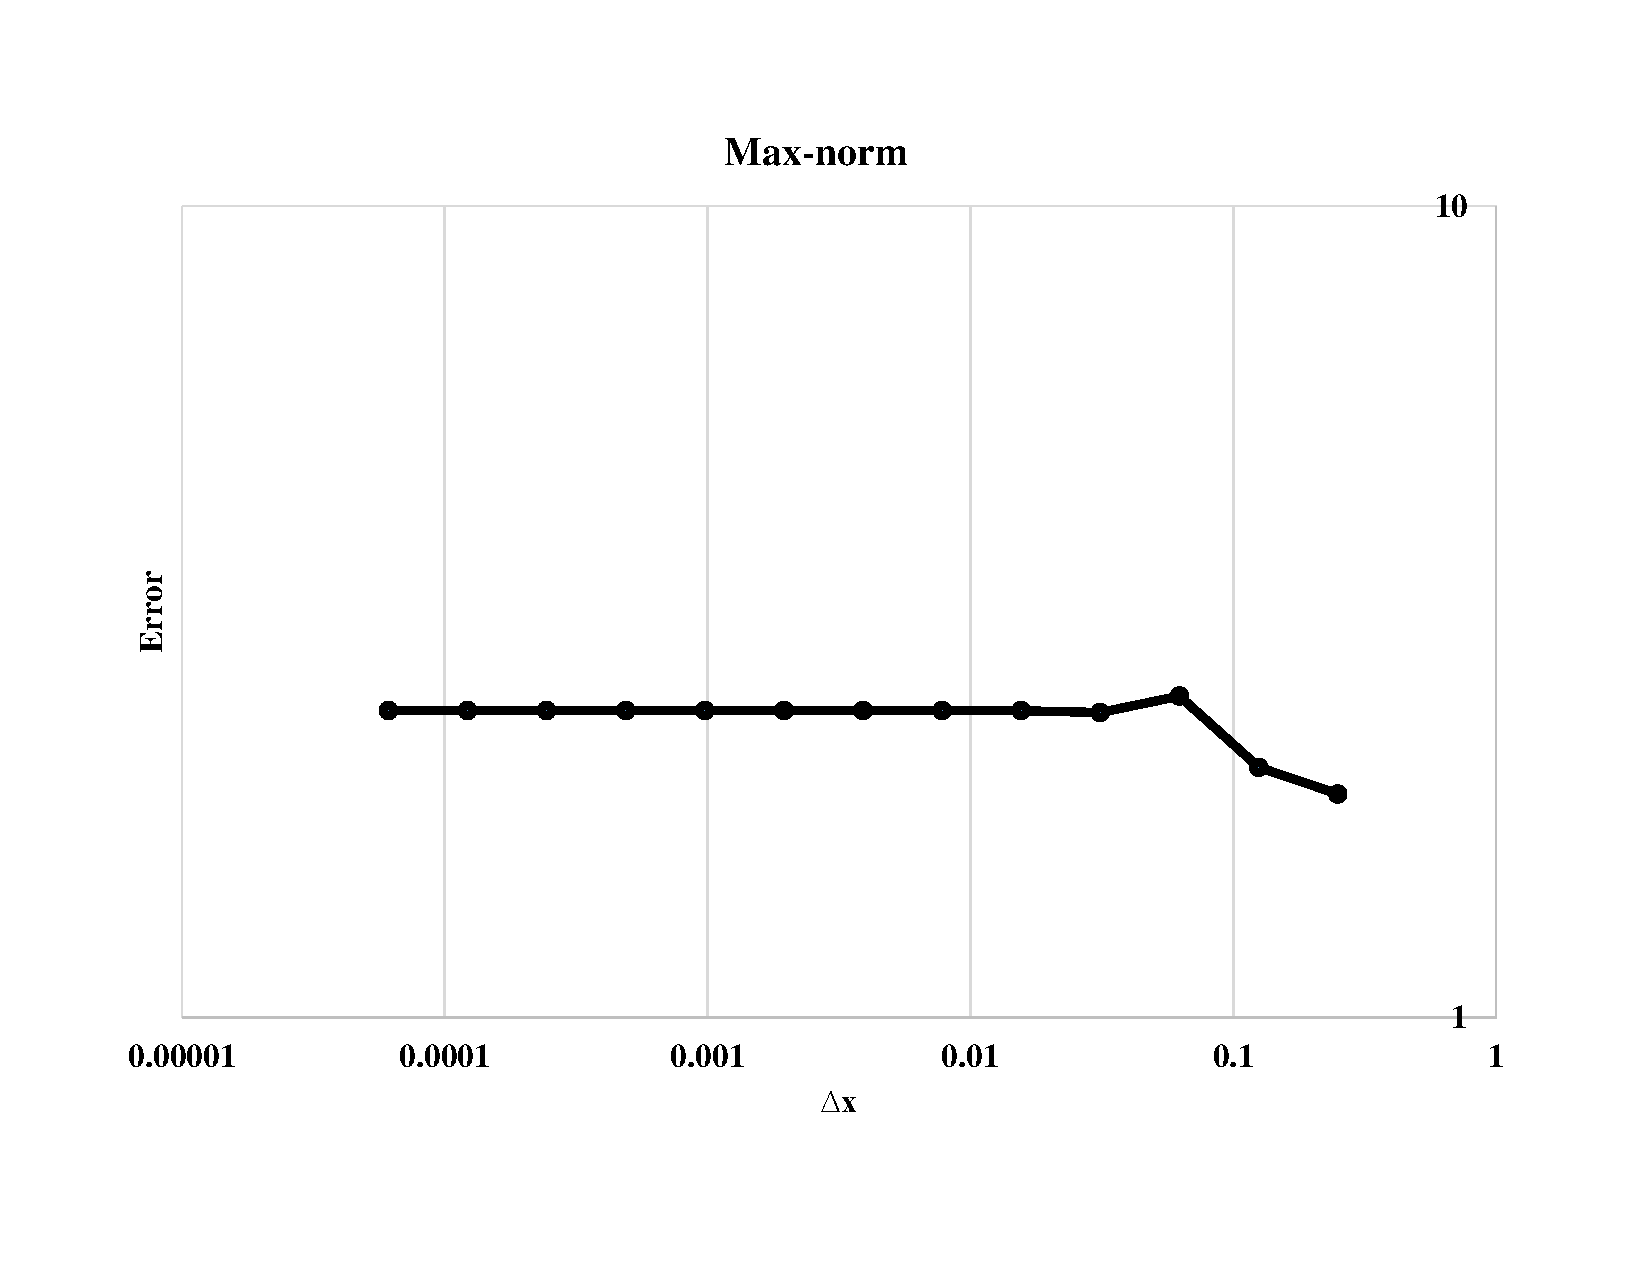
\includegraphics[width=0.3\textwidth]{fig/LW_NonSm_max.pdf}}   
  \caption{The rate convergence in 1-norm (first column),2-norm (second column) and max-norm (third column) for smooth (first two rows) and discontinuous (last two rows) initial condition using upwinding and \protect{\lw} scheme to solve the 1d advection equation.}
   \label{fig:converge}
\end{figure} 